\documentclass[12pt]{article}
\usepackage{amssymb,mathtools, systeme}
\usepackage[margin=1in]{geometry}
\usepackage{fancyhdr}
\usepackage{circuitikz}
\usepackage{graphicx}
\graphicspath{ {./Figures/} }
\usepackage{amsmath}
\usepackage{ragged2e}
\usepackage{subcaption} 
\usepackage{float}
\usepackage{cancel}
\usepackage{siunitx}
\usepackage{bbm}
\pagestyle{fancy}
\usepackage[shortlabels]{enumitem}
\usepackage{mathtools}
\makeatletter
\renewcommand*\env@matrix[1][\arraystretch]{%
  \edef\arraystretch{#1}%
  \hskip -\arraycolsep
  \let\@ifnextchar\new@ifnextchar
  \array{*\c@MaxMatrixCols c}}
\makeatother
\newcommand*{\permcomb}[4][0mu]{{{}^{#3}\mkern#1#2_{#4}}}
\newcommand*{\Comb}[2]{{}^{#1}C_{#2}}%
\DeclarePairedDelimiter\ceil{\lceil}{\rceil}
\DeclarePairedDelimiter\floor{\lfloor}{\rfloor}
\setlength{\headheight}{15 pt}
\lhead{Georgy Antonov}
\chead{HW 8}
\rhead{Neural Dynamics}

\begin{document}\noindent


\noindent\textbf{Question 1. Linear Neural Field.}
\begin{enumerate}
\item[1.1] We are given the following linear neural field
\begin{equation}
    \tau \dot{u}(x, t) =   -u(x, t) + \int_{-\infty}^{\infty}w(x-x')u(x', t)dx' + s(x, t)
\end{equation}
We assume that the input signal is constant over time and is given by 
\begin{equation}
    s(x) = \text{exp}\left(-\frac{x^2}{4d^2}\right)/(2d\sqrt{\pi})
\end{equation}
and that the interaction kernel is given by the Gabor funciton
\begin{equation}
    w(x) = a\left(\text{exp}\left(-\frac{x^2}{4b^2}\right)\text{cos}(k_{0}x)\right)/(b\sqrt{\pi})
\end{equation}
Note that equation 1 is a partial integro-differential equation. To solve it, we begin by transforming it in $x$ to the 
frequency domain using the Fourier Transform $\mathcal{F}$
\[
    \tau \frac{d\widetilde{u}(\omega, t)}{dt} = -\widetilde{u}(\omega, t) + \widetilde{w}(\omega)\widetilde{u}(\omega, t) + \widetilde{s}(\omega)
\]
and after rearranging we get
\[
    \tau \frac{d\widetilde{u}(\omega, t)}{dt} = (-1 + \widetilde{w}(\omega))\widetilde{u}(\omega, t) + \widetilde{s}(\omega)
\]
This is now a linear inhomogeneous ODE in the Fourier domain. If we further assume that the system has a stable solution that does not depend on time,
we get
\[
    \frac{d\widetilde{u}(\omega)}{dt} = 0 \implies (-1 + \widetilde{w}(\omega))\widetilde{u}(\omega) + \widetilde{s}(\omega) = 0
\]
Therefore, we obtain the solution in the Fourier domain
\[
    \widetilde{u}(\omega, \infty) = \frac{\widetilde{s}(\omega)}{1 - \widetilde{w}(\omega)}
\]
\item[1.2] Note that both the interaction kernel and input terms are Gaussians, and hence their Fourier Transforms are 
\[
    \widetilde{s}(\omega) = \mathcal{F}[s](\omega) =  \frac{\text{exp}(-1/4d^{2}\omega^{2})}{2\sqrt{2\pi}}
\]
\begin{align*}
    \widetilde{w}(\omega) = \mathcal{F}[w](\omega) &= \frac{a}{b\sqrt{\pi}}\int_{-\infty}^{\infty}\text{exp}\left(-\frac{x^2}{4b^{2}}\right)\text{cos}(k_{0}x)e^{-i\omega x}dx\\
                           &= \frac{a}{2b\sqrt{\pi}}\int_{-\infty}^{\infty}\text{exp}\left(-\frac{x^2}{4b^{2}}\right)(e^{ik_{0}x}+e^{-ik_{0}x})e^{-i\omega x}dx\\
                           &= \frac{a}{2b\sqrt{\pi}}\left( \text{exp}\left(-\frac{(x-k_{0})^2}{4b^{2}}\right) + \text{exp}\left(-\frac{(x+k_{0})^2}{4b^{2}}\right)\right)
\end{align*}
\item[1.3] As can be seen for the kernel in the frequency domain, parameter $a$ controls the power at frequency $k_0$. Thus, in the original spatial domain, the $a$ parameter controls the interaction strength. 
Plots of the kernel both in spatial and frequency domains are shown below. 
\begin{figure}[H]
    \centering
    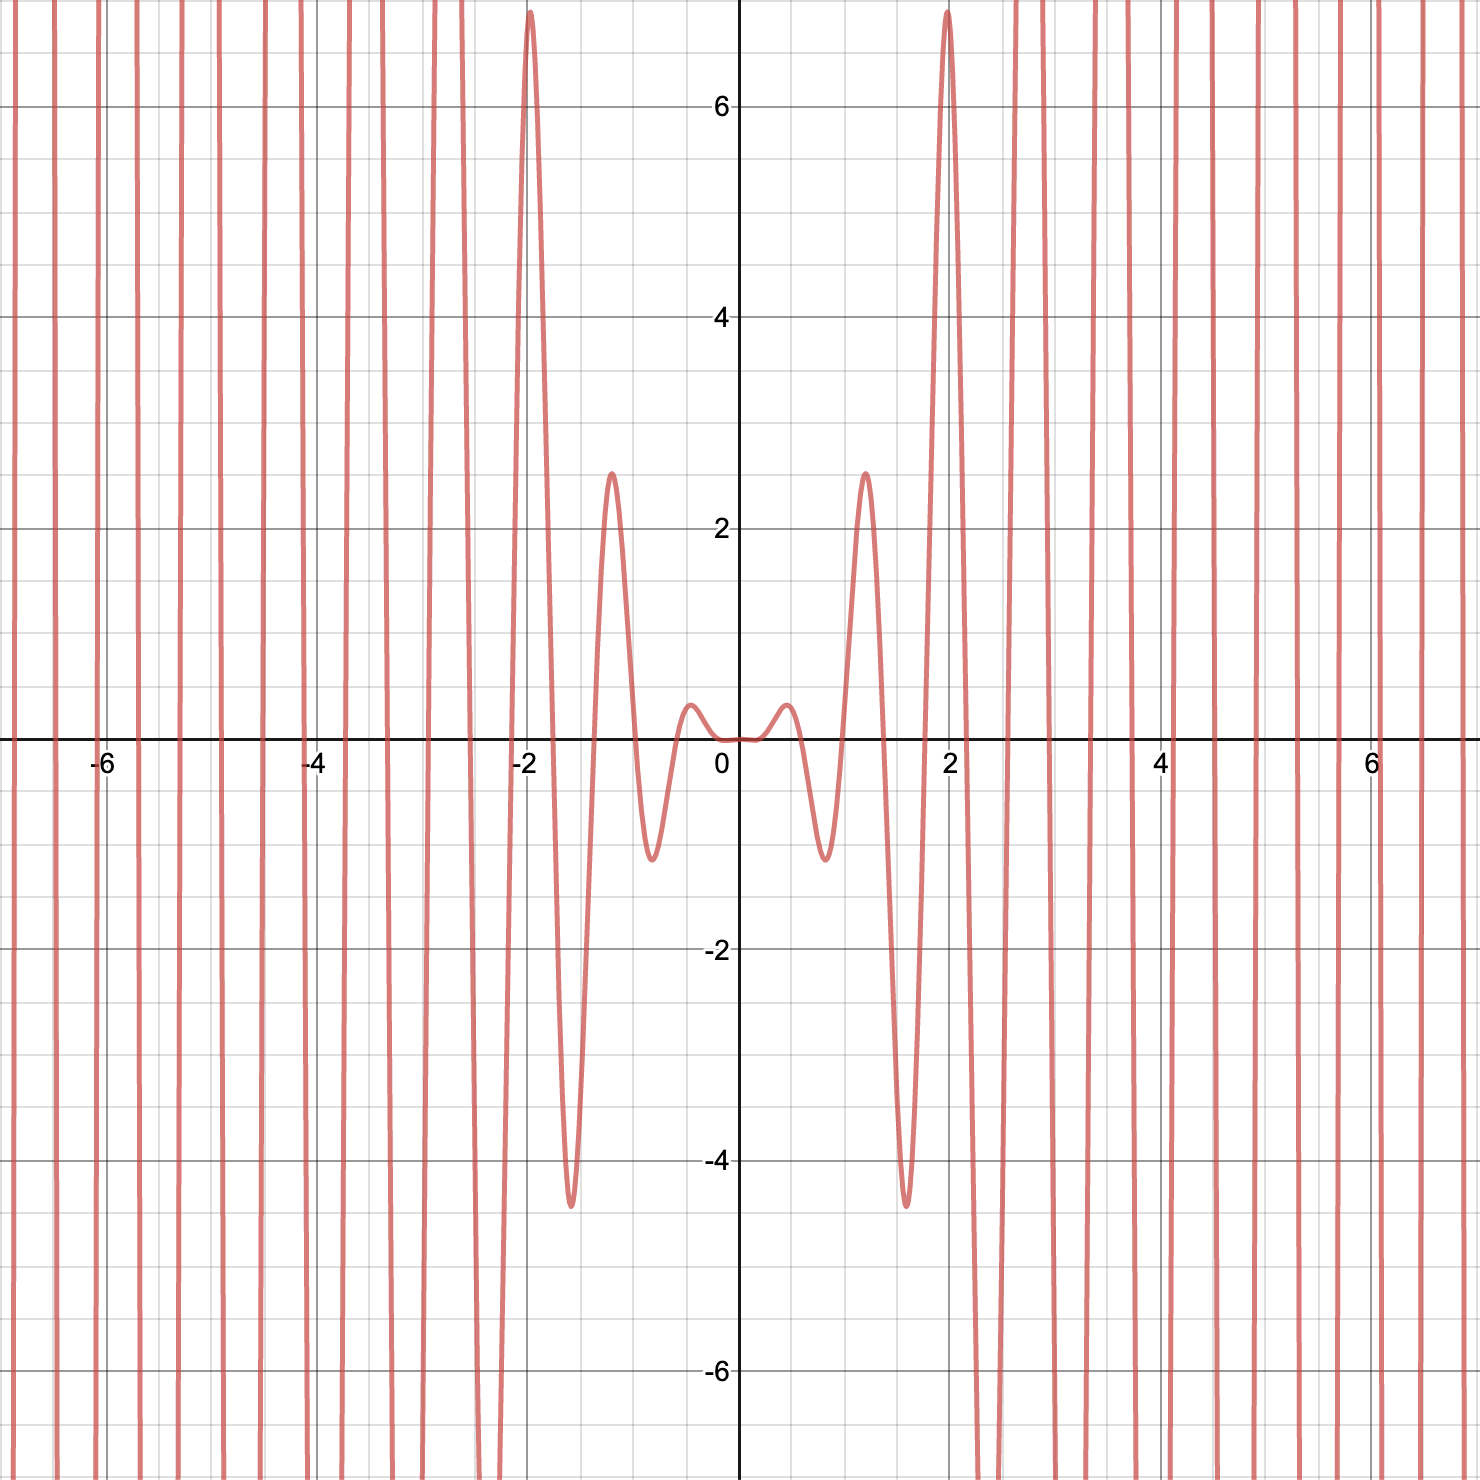
\includegraphics[width=0.7\textwidth]{./k8a1.png}
    \caption{Interaction kernel in the spatial domain for $k=8$ and $a=1$.}
\end{figure}
\begin{figure}[H]
    \centering
    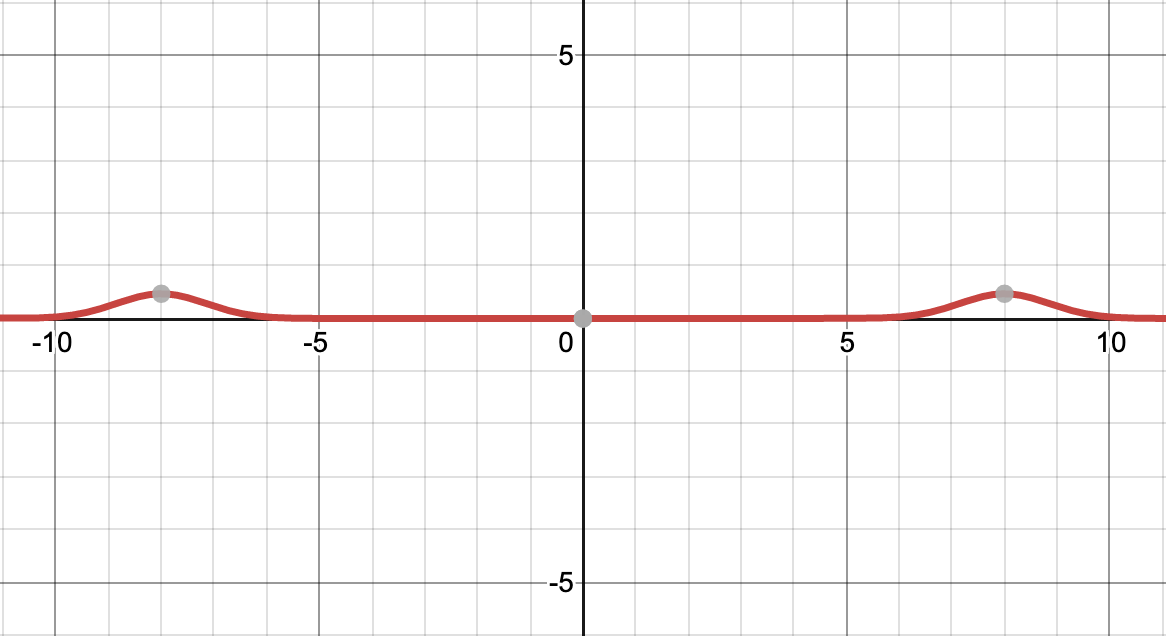
\includegraphics[width=0.7\textwidth]{./a1.png}
    \caption{Interaction kernel in the frequency domain for $k=8$ and $a=1$.}
\end{figure}
\begin{figure}[H]
    \centering
    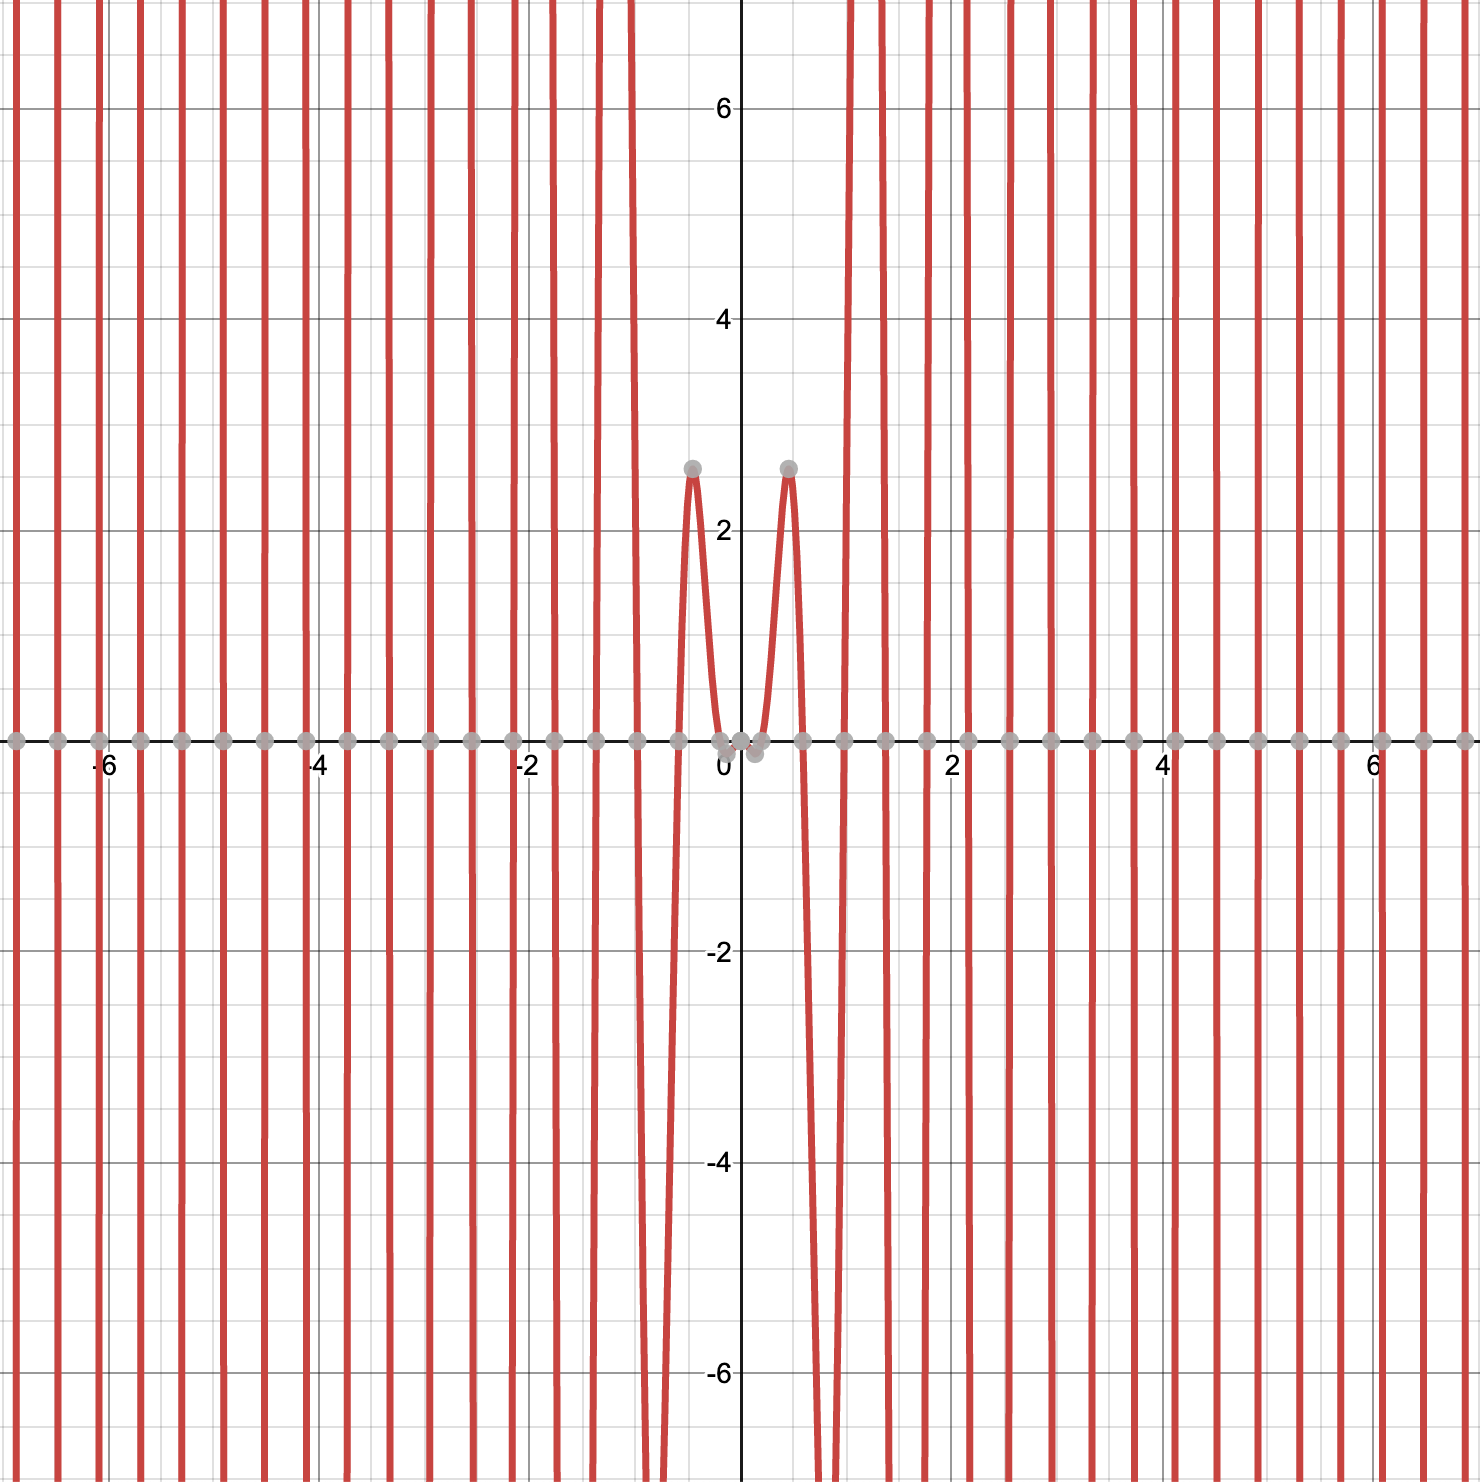
\includegraphics[width=0.7\textwidth]{./k8a8.png}
    \caption{Interaction kernel in the spatial domain for $k=8$ and $a=8$.}
\end{figure}
\begin{figure}[H]
    \centering
    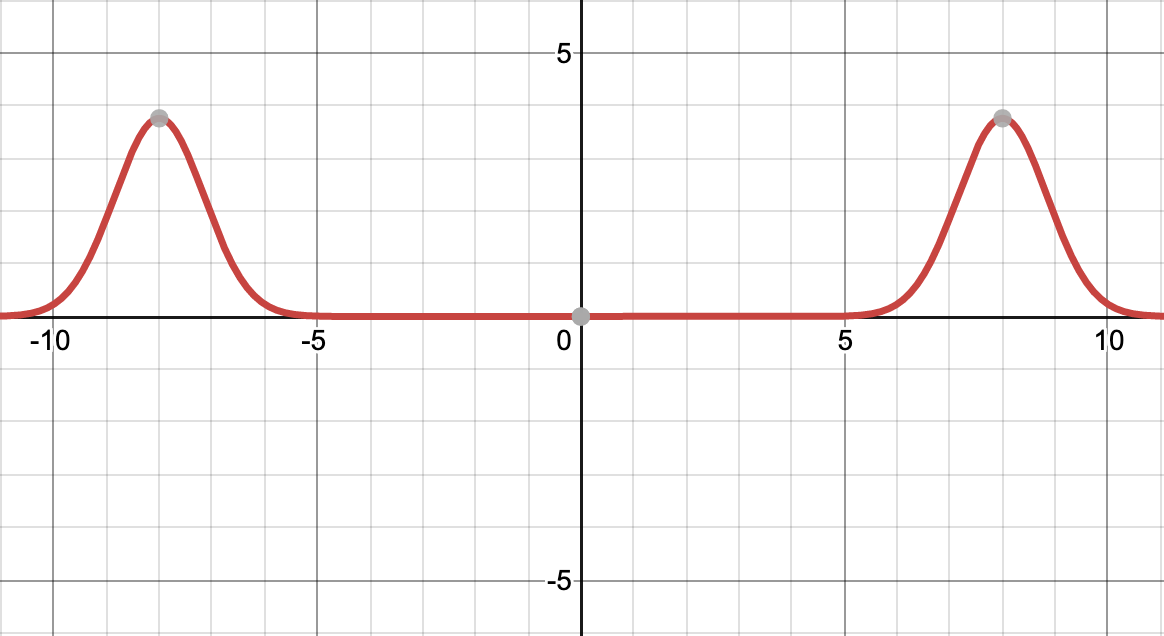
\includegraphics[width=0.7\textwidth]{./a8.png}
    \caption{Interaction kernel in the frequency domain for $k=8$ and $a=8$.}
\end{figure}
Therefore, for $a$ approaching 1 from below we would expect an increasing effect from nearby neurons in the field.
\item[1.4] Now, we simulate the neural field equation by approximating the integral as a Riemann sum
\[
    \int_{A}^{B}f(x)dx \approx \sum_{i=0}^{N} f(x_{i})\Delta x
\]   
with $x_{i} = A + i\Delta x$ and $\Delta x=(B-A)/N$. Thus, we now have
\[
    \tau \dot{u}(x, t) =   -u(x, t) + \sum_{i=0}^{N} \big[ w(x-x_{i})u(x_{i}, t)\Delta x \big] + s(x, t)
\]
We also need to make use of the Forward Euler method to approximate the derivative. Therefore, we finally obtain

\[
    u(x, t+\Delta t) =  u(x, t) + \frac{\Delta t}{\tau}\left(-u(x, t) + \sum_{i=0}^{N} \big[ w(x-x_{i})u(x_{i}, t)\Delta x \big] + s(x, t)\right)
\]

The simulation parameters are as follows
\begin{itemize}
    \item $A = 10$
    \item $B = -10$
    \item $N \geq 200$
    \item $\tau = 10$
    \item $a = 1$
    \item $b=0.6$
    \item $d=2$
    \item $k_{0}=4$
\end{itemize}
The result of the simulation appears in Figure 5. We can see a stationary solution emerging as a localised peak of activity centred at $x=0$.
\begin{figure}[H]
    \centering
    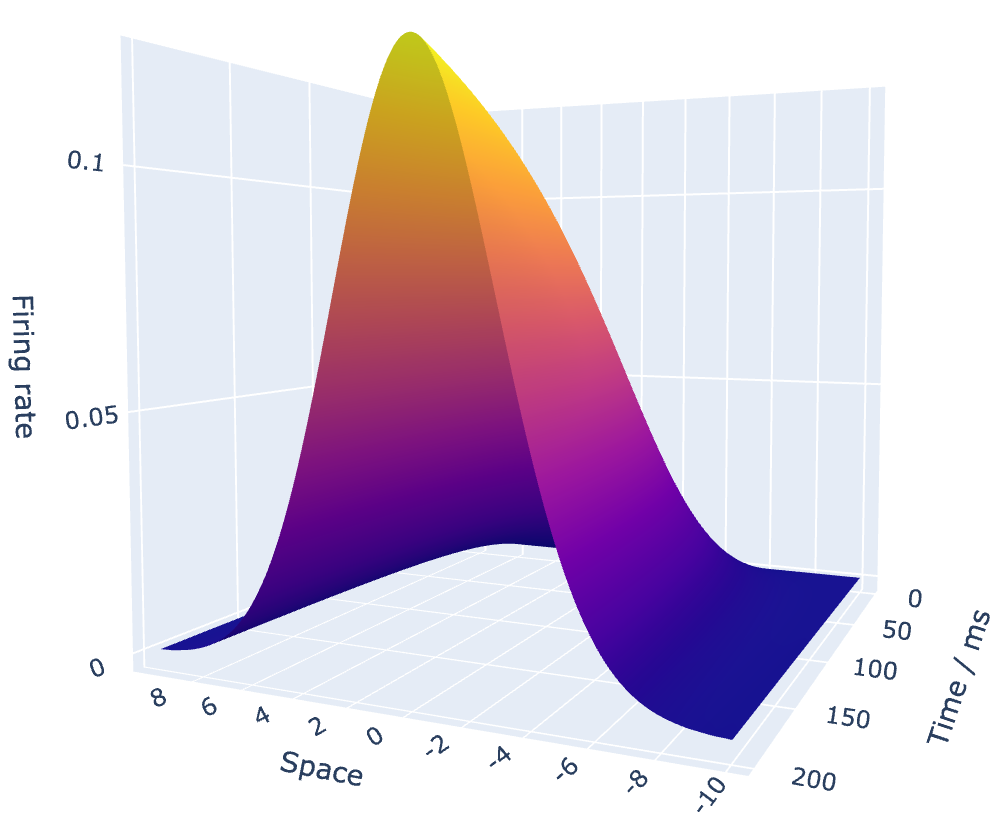
\includegraphics[width=0.9\textwidth]{./figure5.png}
    \caption{Dynamics of the linear neural field defined by equation 1.}
\end{figure}
We can also add a small amount of Gaussian noise to the input signal. This result is shown in Figure 6 for $\sigma^{2}(s(x))=0.01^2$.
With the noise added, the solution remains stable albeit with minor perturbations.
\begin{figure}[H]
    \centering
    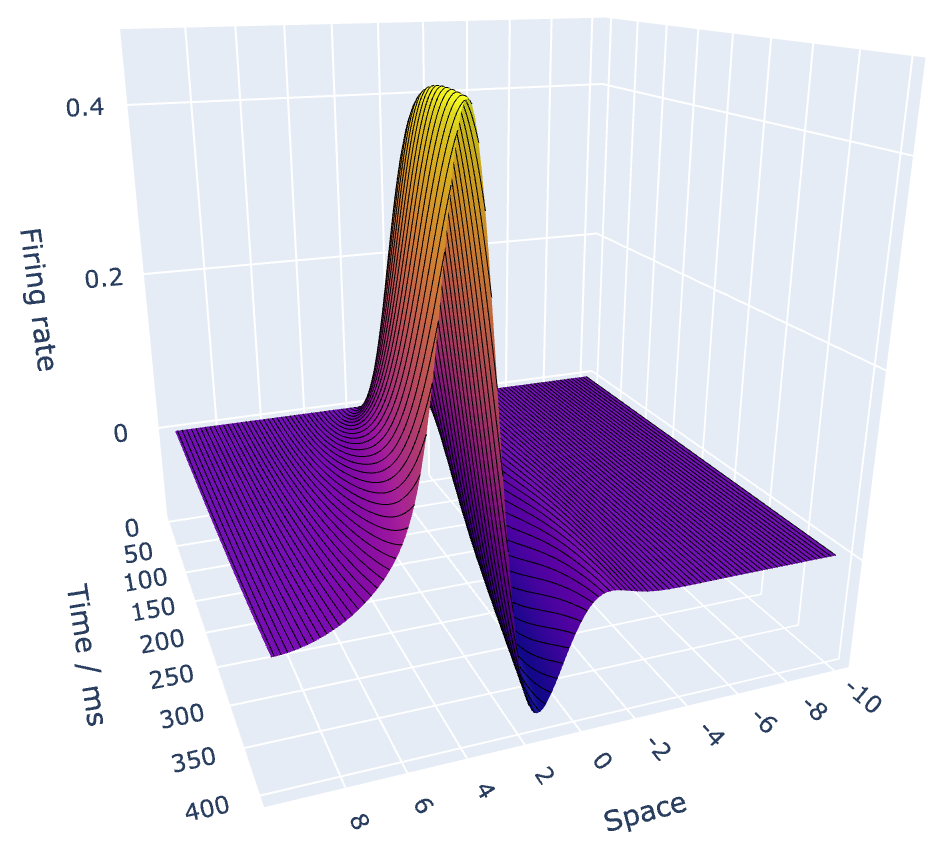
\includegraphics[width=0.9\textwidth]{./figure6.png}
    \caption{Same as in Fig. 1 but with added Gaussian noise.}
\end{figure}
Now, let us change the interaction kernel parameter $a$ keeping the same noise level as before. The results for $a=0.7$
and $a=1.5$ appear in Figures 7 \& 8, repsectively. It can be clearly seen that the $a$ parameter influences the system's 
sensitivity to noise. With a higher value of $a$, the solution looks noisier. 
\begin{figure}[H]
    \centering
    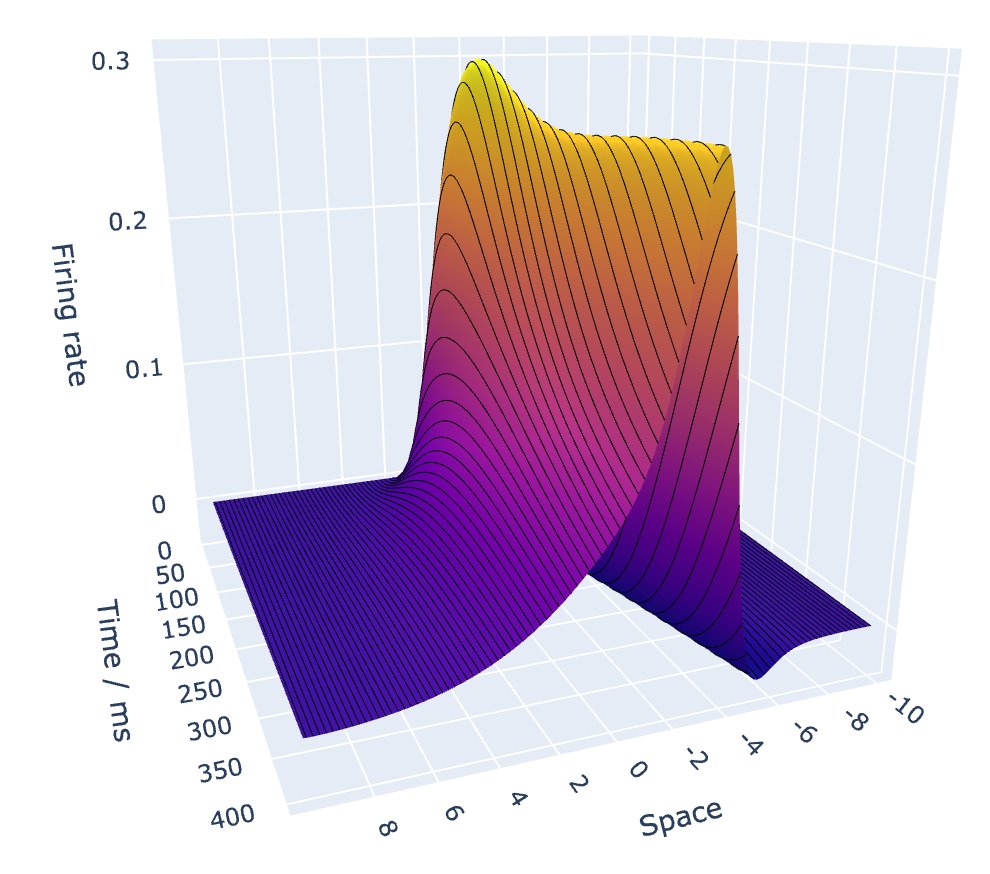
\includegraphics[width=0.9\textwidth]{./figure7.png}
    \caption{Same as in Fig. 1 but with added Gaussian noise and $a=0.7$.}
\end{figure}
\begin{figure}[H]
    \centering
    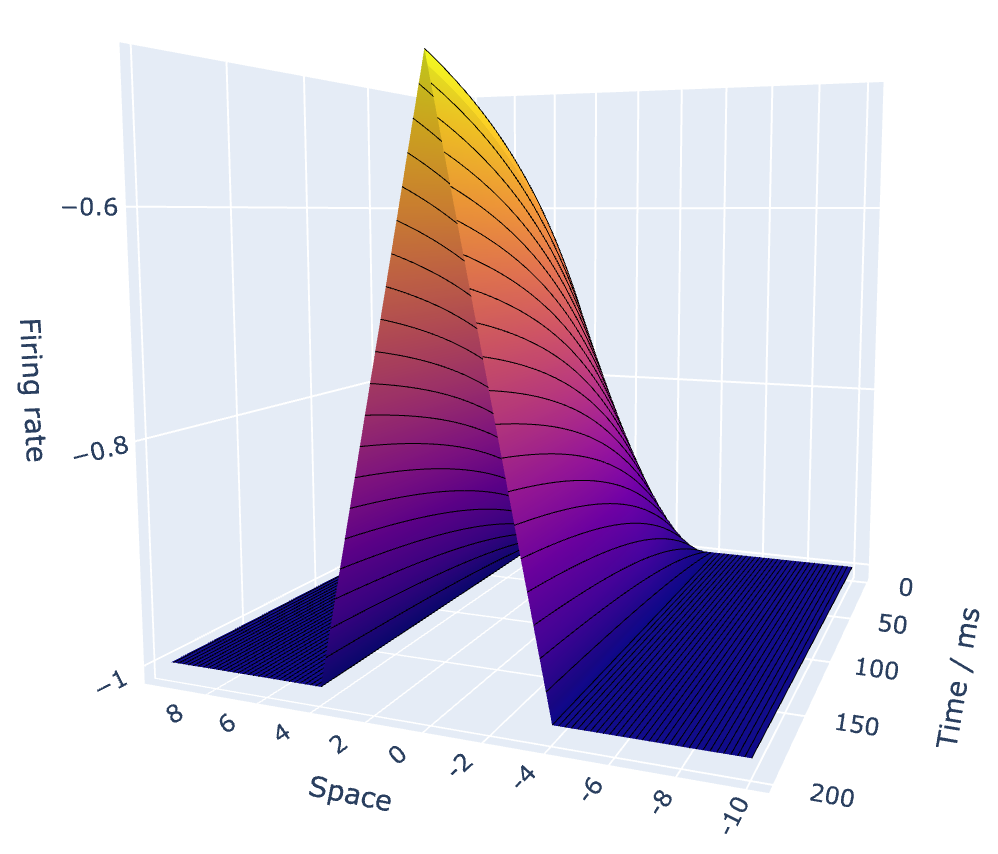
\includegraphics[width=0.9\textwidth]{./figure8.png}
    \caption{Same as in Fig. 1 but with added Gaussian noise and $a=1.5$.}
\end{figure}
Finally, let us discard the noise and keep $a=1$ but now we set $k=8$. This result is shown in figure 9. A higher value of $k$ stretches the solution upwards. With even 
increasing k, the peak becomes higher and boundaries get narrower. This is because k controls the kernel width.
\begin{figure}[H]
    \centering
    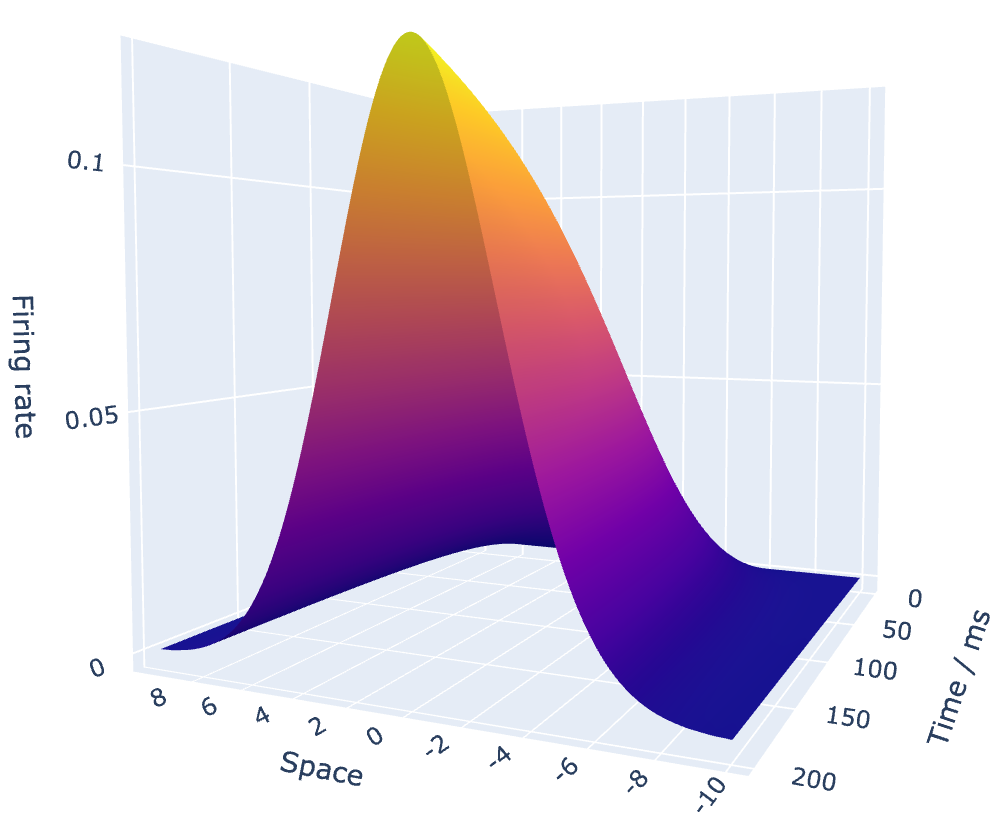
\includegraphics[width=0.9\textwidth]{./figure9.png}
    \caption{Same as in Fig. 1 but with $k=8$.}
\end{figure}
\item[1.5] We can define a Green's function $g(x, t)$ for the neural field that describes its response to a delta input signal of the form $s(x,t) = \delta(x)\delta(t)$. 
 If the function is know, then the response of the filed to $s(x, t)$ is characterised by
 \[
    u(x, t) = \int_{-\infty}^{\infty} \int_{-\infty}^{\infty} g(x-x', t-t')s(x', t')dx'dt'
 \]
Note that we can apply a 2D Fourier Transform to the above equation (i.e. transform both space and time) to obtain $\mathcal{F}[g](k, \omega)$.
First, we transorm the spatial domain (using the convolution theorem)
\[
    \widetilde{u}(k, t) = \int_{-\infty}^{\infty} \widetilde{g}(k, t-t')\widetilde{s}(k, t')dt'
\]
Now, we transform the temporal domain, again applying the convolution theorem
\[
    \mathcal{F}[\tilde{u}](k, \omega) = \mathcal{F}[\tilde{g}](k, \omega)\mathcal{F}[\tilde{s}](k, \omega)
\]
Hence, the 2D Fourier Transform of the Green's function of our neural field is
\[
    \mathcal{F}[\tilde{g}](k, \omega) = \frac{\mathcal{F}[\tilde{u}](k, \omega)}{\mathcal{F}[\tilde{s}](k, \omega)}
\]
\item[1.6] We now assume a different interaction kernel $w(x)$ given by
\[
    w(x) = e^{-c|x|}\text{sign}(x)  
\] 
where $c>0$ and a time-dependent stimulus of the form
\[
    s(x, t) = c\,\text{exp}\left(-\frac{(x-vt)^{2}}{4d_{1}^{2}}\right)/(2d_{1}\sqrt{\pi})
\]
where $v$ is the stimulus peak travelling speed. We run the simulation with the following parameters
\begin{itemize}
    \item $c=1$
    \item $d_{1}=0.5$
    \item $v=0.1$
\end{itemize}
The result is reported in Figure 10.
\begin{figure}[H]
    \centering
    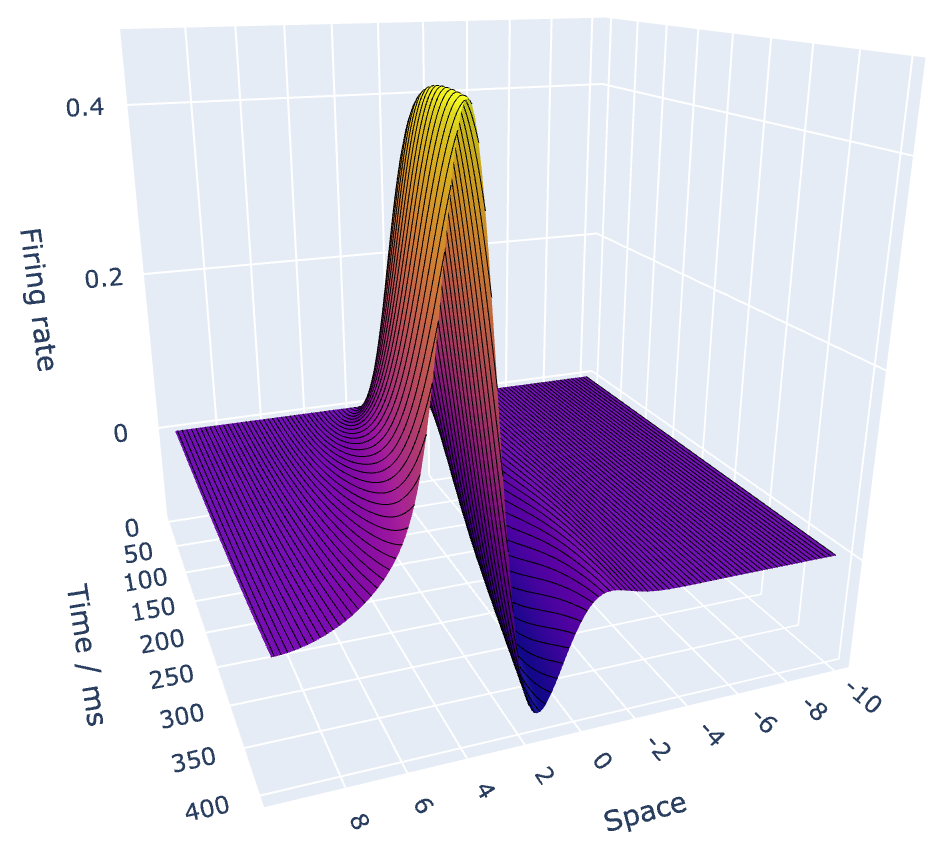
\includegraphics[width=0.9\textwidth]{./figure10.png}
    \caption{Linear neural field dynamics with different interaction kernel and input.}
\end{figure}
Now, if we change the stimulus travelling speed to $v=-0.1$, we yeild what is shown in Figure 11.
\begin{figure}[H]
    \centering
    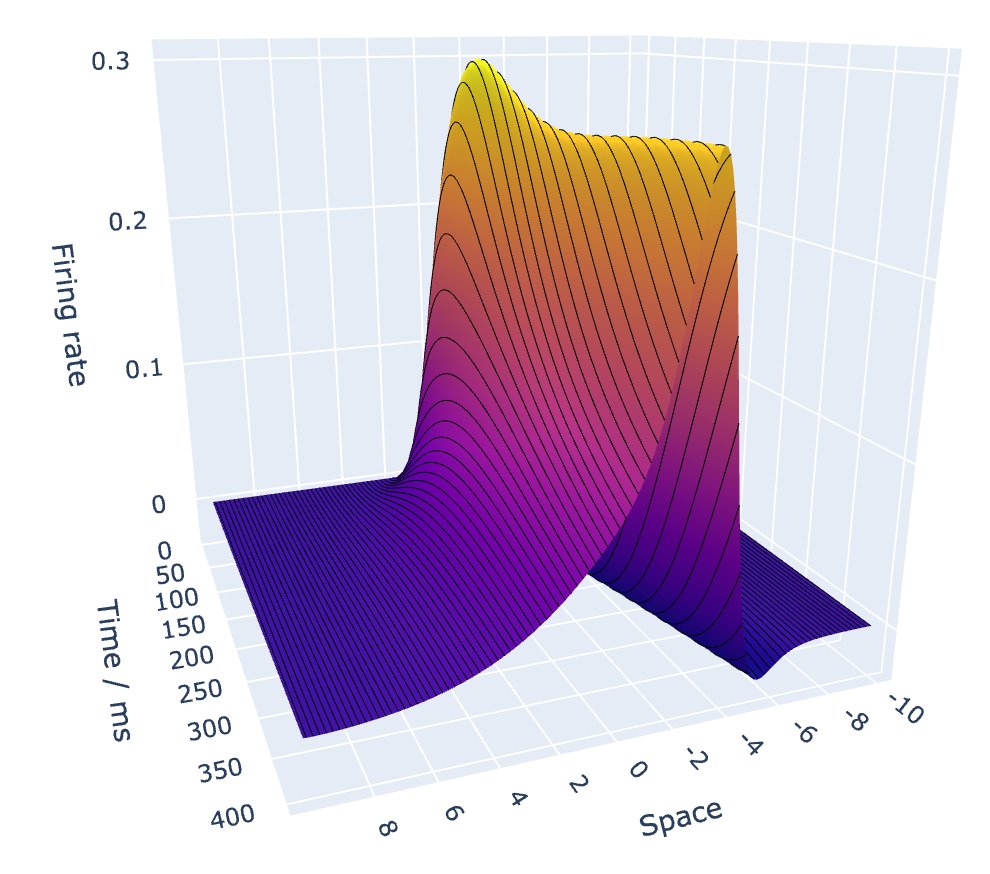
\includegraphics[width=0.9\textwidth]{./figure11.png}
    \caption{Same as in Fig. 6 but a negative stimulus speed.}
\end{figure}
The solution turns, or changes it's direction depending on the input velocity. Hence, this implies potential direction selectivity for the neural field computations. 
\item[1.7] We are required to compute the optimal input speed that leads to the highest output amplitude in the field assuming $|c| << k$.
Recall that our solution in the Fourier domain is
\[
    \widetilde{u}(\omega, \infty) = \frac{\widetilde{s}(\omega)}{1 - \widetilde{w}(\omega)}  
\] 
This time, we also have
\begin{align*}
    \widetilde{w}(\omega) &= \mathcal{F}[w](\omega) = \frac{2i\omega}{c^{2}+\omega^{2}}
\end{align*}
\end{enumerate}

\newpage
\noindent\textbf{Question 2. Noninear Neural Field.}
\begin{enumerate}
\item[2.1] We are given a neural field of Amari type which is described by the following equation
\begin{equation}
    \tau \dot{u}(x, t) =   -u(x, t) + \int_{-\infty}^{\infty}w(x-x')\mathbbm{1}[u(x', t)]dx' + s(x, t) - h
\end{equation}
We assume the resting level parameter, $h=1$, and that both the input and recurrent interaction kernel are given by the 
following piecewise linear functions
\[
    s(x)=\begin{cases}
        C(1-|x|/d), & |x| \leq d\\
        0, & \text{otherwise}
    \end{cases}  
\]
\[
    w(x)=\begin{cases}
        A, & |x| \leq a\\
        -B, & a \leq |x| \leq b\\
        0, & \text{otherwise}
    \end{cases} 
\]
To simulate this neural field, similarly to Question 1, we use the Forward Euler approximation and we also 
express the convolution integral as a Riemann sum
\[
    \dot{u}(x, t+\Delta t) = u(x, t) + \frac{\Delta t}{\tau}\left(-u(x, t) + \sum_{i=0}^{N}\big[ w(x-x_{i})\mathbbm{1}[u(x_{i}, t)]\Delta x \big] + s(x, t) - h\right)
\]
Initially, we use the following parameters
\begin{itemize}
    \item $A=3$
    \item $B=2$
    \item $C=0.6$
    \item $a=1$
    \item $b=3$
    \item $d=4$
    \item $h=1$
\end{itemize}
The result of the simulation with the initial condition $u(x, 0)=-h$ is shown in Figure 12.
\begin{figure}[H]
    \centering
    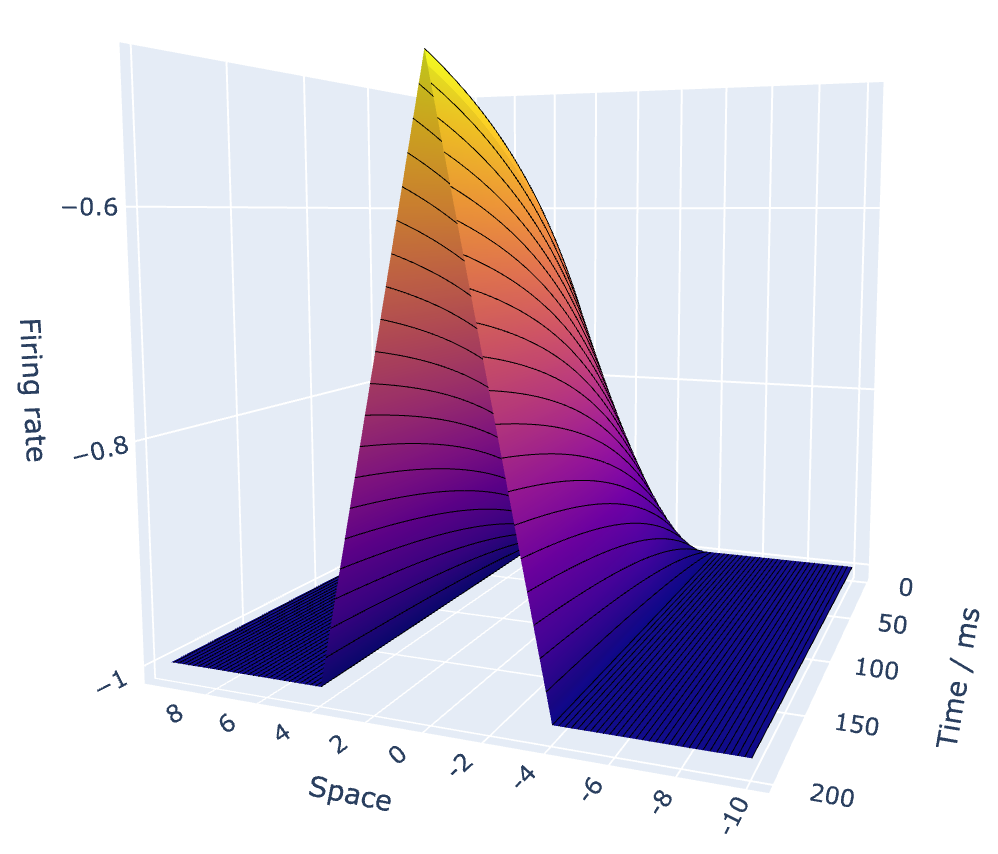
\includegraphics[width=0.9\textwidth]{./figure12.png}
    \caption{Dynamics of the nonlinear neural field defined by equation 4.}
\end{figure}
Now, we run another simulation but this time with a different initial condition, $u(x, 0)=3.3s(x)-h$. This simulation appears in Figure 9.
The apparent change can be explained by the fact that now our kernel starts to 'act' in all 3 modes given by the definition. Hence, we see 3 stable solutions.
\begin{figure}[H]
    \centering
    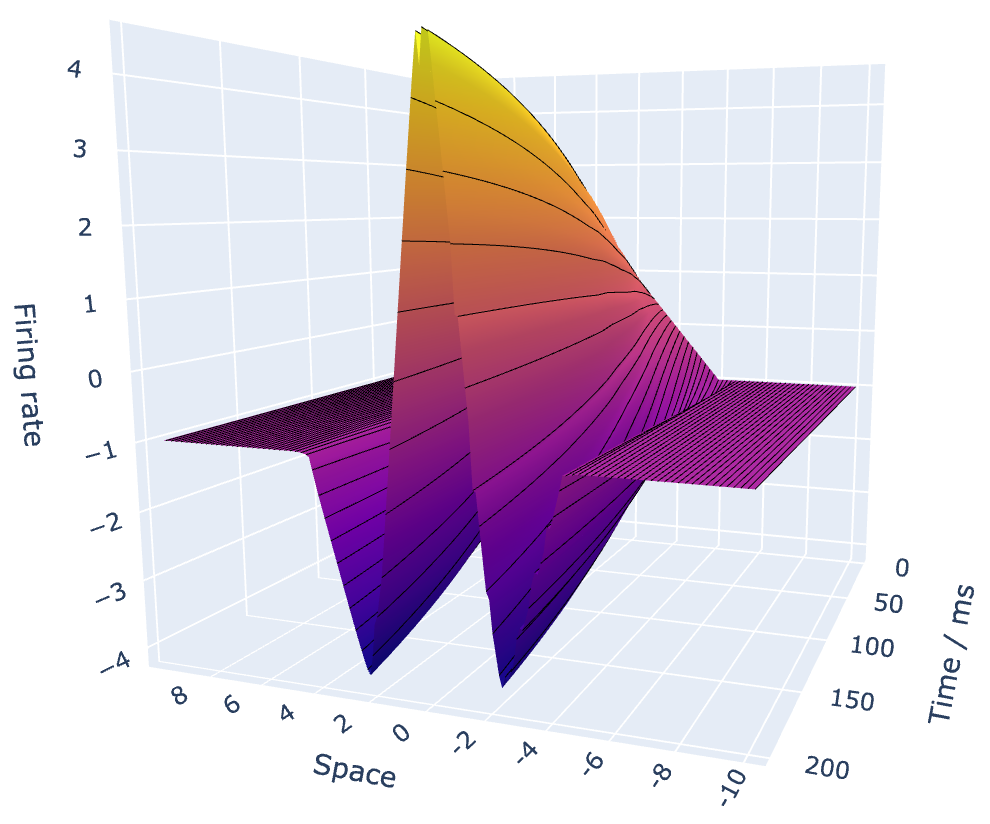
\includegraphics[width=0.9\textwidth]{./figure13.png}
    \caption{Same as in Figure 12 but with the initial condition $u(x, 0)=3.3s(x)-h$.}
\end{figure}
Finally, we reduce the strength of the interaction kernel by one order of magnitude and run the simulation again with the remaining parameters as before.
This simulation result is shown in Figure 14.
\begin{figure}[H]
    \centering
    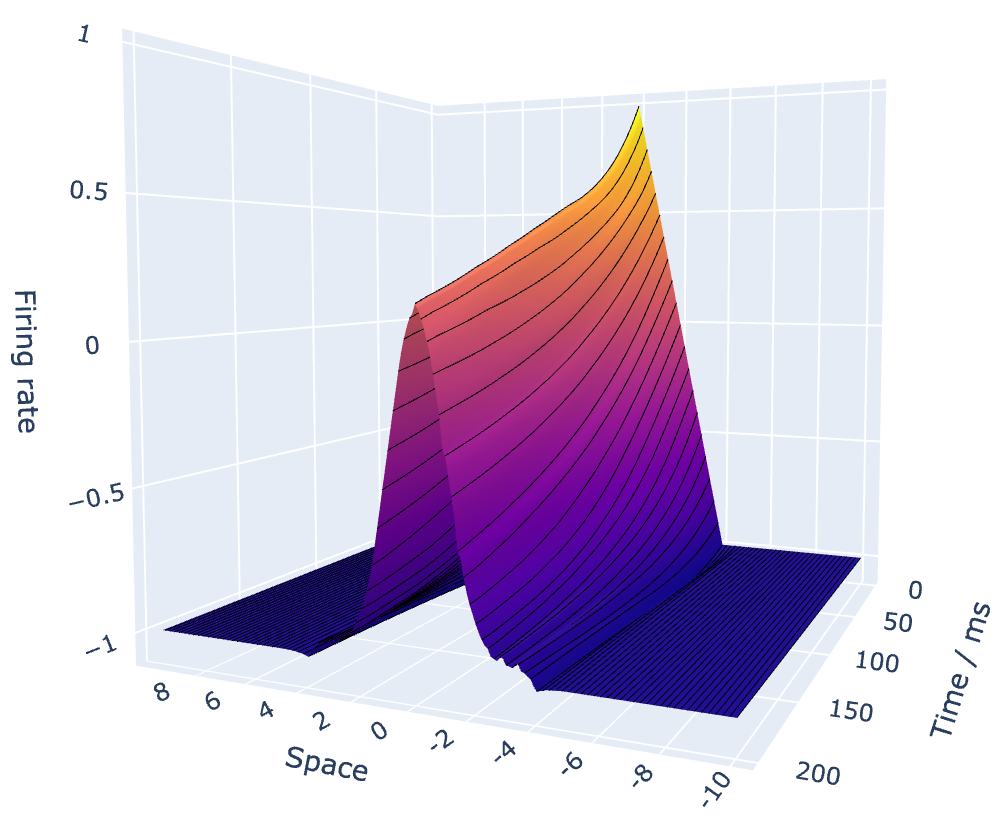
\includegraphics[width=0.9\textwidth]{./figure14.png}
    \caption{Same as in Figure 13 but with the interaction kernel $w(x)$ weakend by one order of magnitude.}
\end{figure}
The stationary solution appears at a firing rate of $\approx 0.3$, which is $0.1w(x)$ for the initial condition 
used in this simulation.
\item[2.2] As can be clearly seen from Figure 12, we have a localised activation peak
\[
    u^{\star}(x)=\begin{cases}
                \geq -h, & x_{1} \leq x \leq x_{2}\\
                -h, & \text{otherwise}
            \end{cases} 
\] 
Hence, we can express the field dynamics within the peak by
\[
    \tau \frac{\partial u(x, t)}{\partial t} = -u(x, t) + \int_{x_{1}(t)}^{x_{2}(t)}w(x-x')dx' + s(x) - h
\]
where $x_{1}(t)$ and $x_{2}(t)$ are time-dependent boundaries of the peak. We can further simplify this to
\[
    \tau \frac{\partial u(x, t)}{\partial t} = -u(x, t) - W(x-x_{2}(t)) + W(x-x_{1}(t)) + s(x) - h
\]
where 
\[
    W(x) = \int_{0}^{x}w(x')dx'
\]
Thus, our stationary solution is
\[
    u^{\star}(x) = W(x-x_{1}^{\star}(t)) - W(x-x_{2}^{\star}(t)) + s(x) - h
\]
At the boundaries of our excited region, we have $u^{\star}(x) = -1$. Hence, this implies the following system with $a=x_{2}-x_{1}$
\begin{align*}
   &- W(x_{1}^{\star}(t)-x_{1}^{\star}(t)) + W(x_{1}^{\star}(t)-x_{2}^{\star}(t)) = W(-a^{\star}) = s(x_{1}^{\star})-h\\
   &- W(x_{2}^{\star}(t)-x_{1}^{\star}(t)) + W(x_{2}^{\star}(t)-x_{2}^{\star}(t)) = -W(a^{\star}) = s(x_{2}^{\star})-h
\end{align*}
For spatially constant input, the above equations are satisfied for the symmetric kernel which fulfills
\[
    W(a^{\star}) + s -h = 0
\]
Now, let us us employ the level-set method to analyse stability at the boundary points
\[
    u(x_{i}, t)=-1 \implies \frac{dx_{i}}{dt} = -\frac{\partial u(x_{i}, t)}{\partial t}/ \frac{\partial u(x_{i}, t)}{\partial x}  
\]
for $i \in \{1, 2\}$. Let us define
\[
 \gamma_{i} \doteq \frac{\partial}{\partial x} u(x_{i}, t)
\]
Substituting into the above we get
\begin{align*}
    \frac{dx_{1}}{dt} &= -\frac{1}{\tau \gamma_{1}}[-W(x_{1}(t)-x_{2}(t)) + s -h]\\
    \frac{dx_{2}}{dt} &= -\frac{1}{\tau \gamma_{2}}[W(x_{2}(t)-x_{1}(t)) + s -h]  
\end{align*}
Note that if we subtract second equation from the first, we get
\[
    \frac{da}{dt} = \frac{1}{\tau}\left( \frac{1}{\gamma_{1}} - \frac{1}{\gamma_{2}} \right)[W(a(t))+s-h]
\]
Since the gamma-tau term is non-negative, this implies asymptotic stability for 
\[
    \frac{dW}{da}\bigg|_{a^{\star}} = w(a^{\star}) < 0
\]
% To analyse the stability of our spatially homogeneous solution, let us first assume no space dependence, i.e.
% \[
%     \tau \frac{du(t)}{dt} =   -u(t) + \int_{-\infty}^{\infty}w(x)\mathbbm{1}[u(t)]dx + s(t) - h
% \] 
% The equation can be further simplified to
% \[
%     \tau \frac{du(t)}{dt} =   -u(t) + \overline{w}(x)\mathbbm{1}[u(t)]dx + s(t) - h
% \]
% with 
% \[
%     \overline{w}(x) = \int w(x)dx
% \]
% This is now a simple DEQ. We can now employ the isocline analysis
% \[
%     \frac{du(t)}{dt} = 0 \implies \frac{h-s(t)+u(t)}{\overline{w}} = \mathbbm{1}[u(t)]
% \]
% Therefore, we obtain the fixed points
% \[
%     u_{0}(t)=\begin{cases}
%         s(t) - h, & u(t) \leq 0\\
%         {\overline{w}} + s(t) - h, & u(t) > 0
%     \end{cases} 
% \]
% Now, we also need to account for spatial perturbations to the stationary points, for the system is spatially dependent. 
% To do that, let us consider a small perturbation $\delta u(x, t)$ around the stationary solution $u(x) \equiv u_{0}$ which is 
% given by linearisation
% \[
%     u(x, t)=u_{0}+\delta u(x, t)
% \]
% which implies the linearised dynamics 
% \[
%     \tau \frac{\partial \delta u(x, t)}{\partial t} = -\delta u(x, t) +   
% \]
\item[2.4] Now we simulate the same neural field with the initial condition $u(x, 0)=3.3s(x)-h$ and the initial interaction kernel;
however, we set the input current to zero (but not for the initial condition). The result is shown in Figure 15. 
\begin{figure}[H]
    \centering
    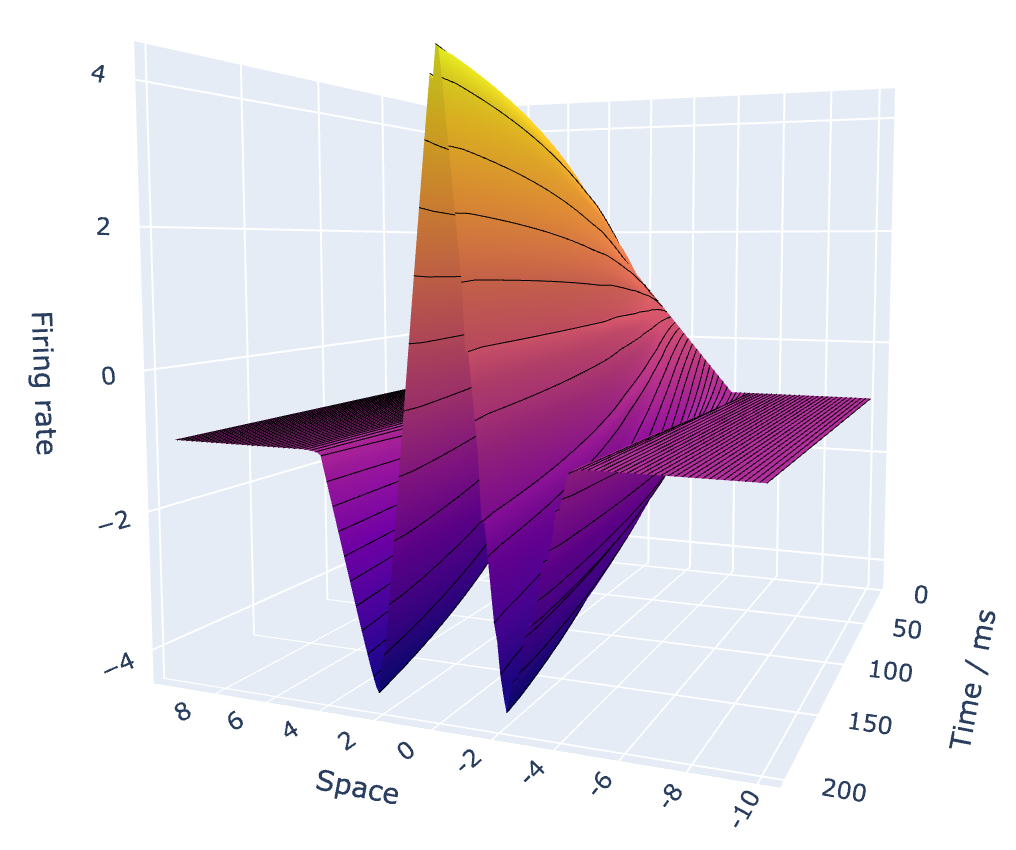
\includegraphics[width=0.9\textwidth]{./figure15.png}
    \caption{Nonlinear neural field dynamics with the initial condition $u(x, 0)=3.3s(x)-h$ and the initial interaction kernel, but no input current.}
\end{figure}
\item[2.5] Finally, we run the simulatiom with the same conditions as above, except that now we add a non-symmetric interaction kernel to our previous kernel, i.e.
effectively we have $w(x)+w_{u}(x)$, where
\[
    w_{u}(x)=\begin{cases}
        0.8x, & |x| \leq b\\
        0, & \text{otherwise}
    \end{cases} 
\] 
The emerging solution appears in Figure 16.
\begin{figure}[H]
    \centering
    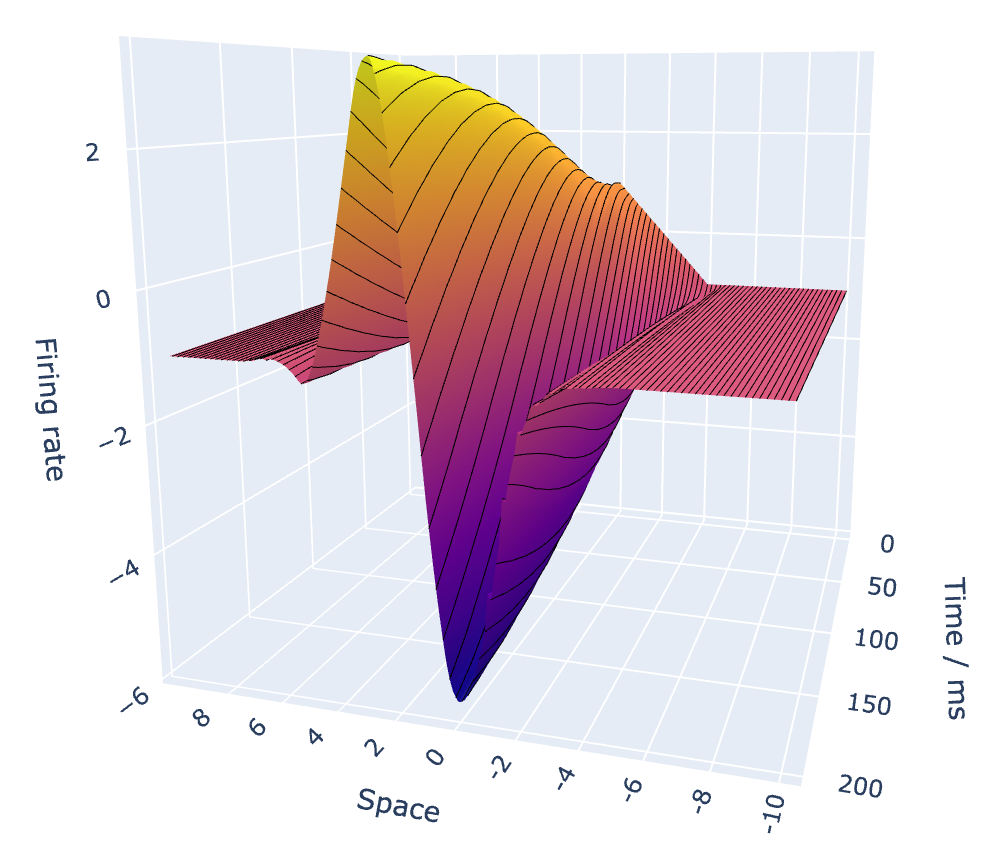
\includegraphics[width=0.9\textwidth]{./figure16.png}
    \caption{Nonlinear neural field dynamics with the initial condition $u(x, 0)=3.3s(x)-h$ and the interaction kernel $w(x)+w_{u}(x)$.}
\end{figure}
\end{enumerate}
\end{document}
